\documentclass[12font]{article}
\title{\textbf{ Block-Diagonalization of Density Matrices — A Consequence of Gauge Theory }}
\author{Chen-Chih Wang  }
\date{\textit{Department of physics, National Tsing Hua University, Hsinchu 30013, Taiwan} \\ (Dated: \today)}
\usepackage[margin=2cm]{geometry}
%\usepackage[fleqn]{amsmath}
%\usepackage{CJK,amsmath}
\usepackage{amsfonts,amssymb}
\usepackage{fancyhdr}
%\pagestyle{fancy}
\usepackage{textcomp}
\usepackage{graphicx}
\usepackage{float}
\usepackage{color}
\usepackage{tikz}
\usepackage{multicol}
\usepackage{threeparttable}
\usepackage{amsthm}
\usepackage{mathtools}
\usepackage{hyperref}
\urlstyle{same}
\usepackage{caption}
\usepackage{subcaption}
\usepackage{dsfont}
\usepackage{comment}
\newtheorem{theorem}{Theorem}[section]
\theoremstyle{definition}
\newtheorem{definition}{Definition}[section]
\newtheorem{lemma}[theorem]{Lemma}
\newtheorem{corollary}{Corollary}[theorem]
\newtheorem{proposition}[theorem]{Proposition}

\numberwithin{equation}{section}

\newcommand{\vac}{\mrm{vac}}
\newcommand{\Bra}[1]{\left\langle #1 \right|}
\newcommand{\Ket}[1]{\left| #1 \right\rangle}
\newcommand{\bra}[1]{\langle #1 |}
\newcommand{\ket}[1]{| #1 \rangle}
\newcommand{\anglelr}[1]{\left\langle #1 \right\rangle}
\newcommand{\sanglelr}[1]{\langle #1 \rangle}
\newcommand{\braket}[2]{\langle #1 | #2 \rangle}
\newcommand{\Bbraket}[2]{\left\langle #1 \right|\left. #2 \right\rangle}
\newcommand{\dif}[1]{\frac{\mathrm{d}}{\mathrm{d}#1}}
\newcommand{\diff}[2]{\frac{\mathrm{d}#1}{\mathrm{d}#2}}
\newcommand{\gd}{\boldsymbol{\nabla}}
\newcommand{\dive}{\boldsymbol{\nabla}\cdot}
\newcommand{\curl}{\boldsymbol{\nabla}\times}
\newcommand{\lr}[1]{\left(  #1  \right)}
\newcommand{\lrm}[1]{\left[  #1  \right]}
\newcommand{\lrg}[1]{\left\{  #1  \right\}}
\newcommand{\abs}[1]{\left|  #1  \right|}
\newcommand{\de}{\partial}
\newcommand{\pdif}[1]{\frac{\partial}{\partial#1}}
\newcommand{\pdiff}[2]{\frac{\partial#1}{\partial#2}}
\newcommand{\mrm}[1]{\mathrm{#1}}
\newcommand{\bo}[1]{\mathbf{#1}}
\newcommand{\bog}[1]{\boldsymbol{#1}}
\newcommand{\vint}[3]{\int_{#1}#2\cdot\mathrm{d}\mathbf{#3}}
\newcommand{\voint}[3]{\oint_{#1}#2\cdot\mathrm{d}\mathbf{#3}}
\newcommand{\Vint}{\int\mrm{d}^3\bo{r}'}
\newcommand{\rr}{\mathbf{r} - \mathbf{r}'}
\newcommand{\arr}{\left|\mathbf{r} - \mathbf{r}'\right|}
\newcommand{\nx}{\hat{\bo{n}}_1}
\newcommand{\ny}{\hat{\bo{n}}_2}
\newcommand{\alert}[1]{{\color{red}#1}}
\newcommand{\alertV}[1]{{\color{violet}#1}}
\newcommand{\Tr}{\mrm{Tr}}
\newcommand{\norm}[1]{\left\lVert#1\right\rVert}

\newcommand{\wordfig}[2]{\begin{minipage}[h]{#1 cm}
	\vspace{0pt}
	\includegraphics[width=\textwidth]{#2}
   \end{minipage}}

\begin{document}
\maketitle
\begin{abstract}
  This note demonstrates how to use the approach and physical picture proposed by Ref.\cite{PRX} to understand the origin of the gauge part of the entanglement entropy given by Yao and Qi. After the discussion, we will see that the gauge part of the entanglement entropy arises from the Gauss law of the gauge theory, which can also be understood as the degree of degeneracies in the entanglement spectrum; While the topological entanglement entropy is given rise by the one-form symmetry characterized by the Wilson loops, which fix the parity of the spectrum, hence the reduction of the degeneracies. 
\end{abstract}

\section{Background}
\begin{figure}[H]
  \centering
  (a)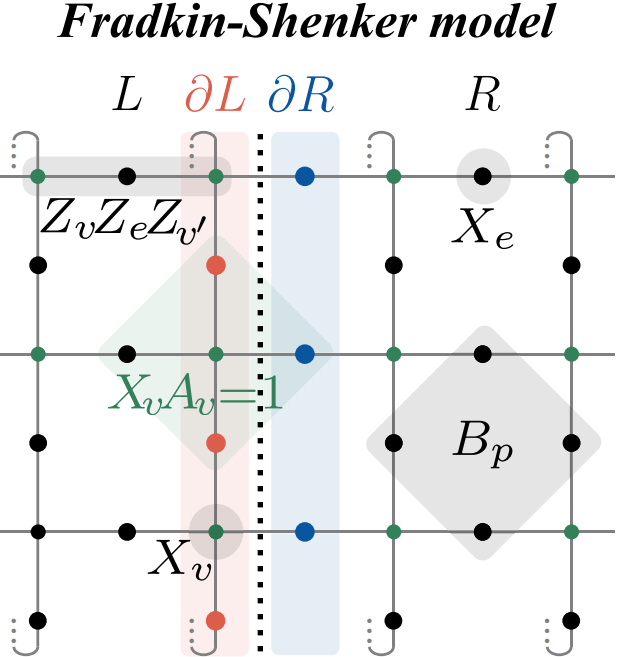
\includegraphics[height=0.12\textheight]{FS-model}
  (b)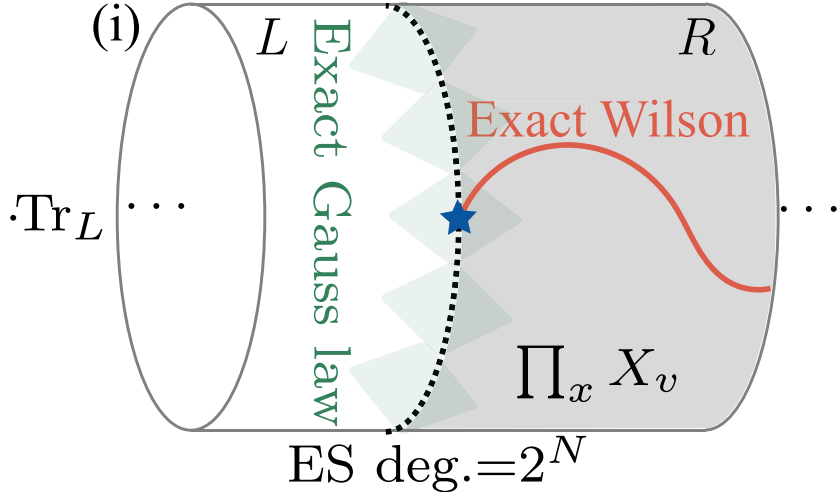
\includegraphics[height=0.12\textheight]{LR-def}
  (c)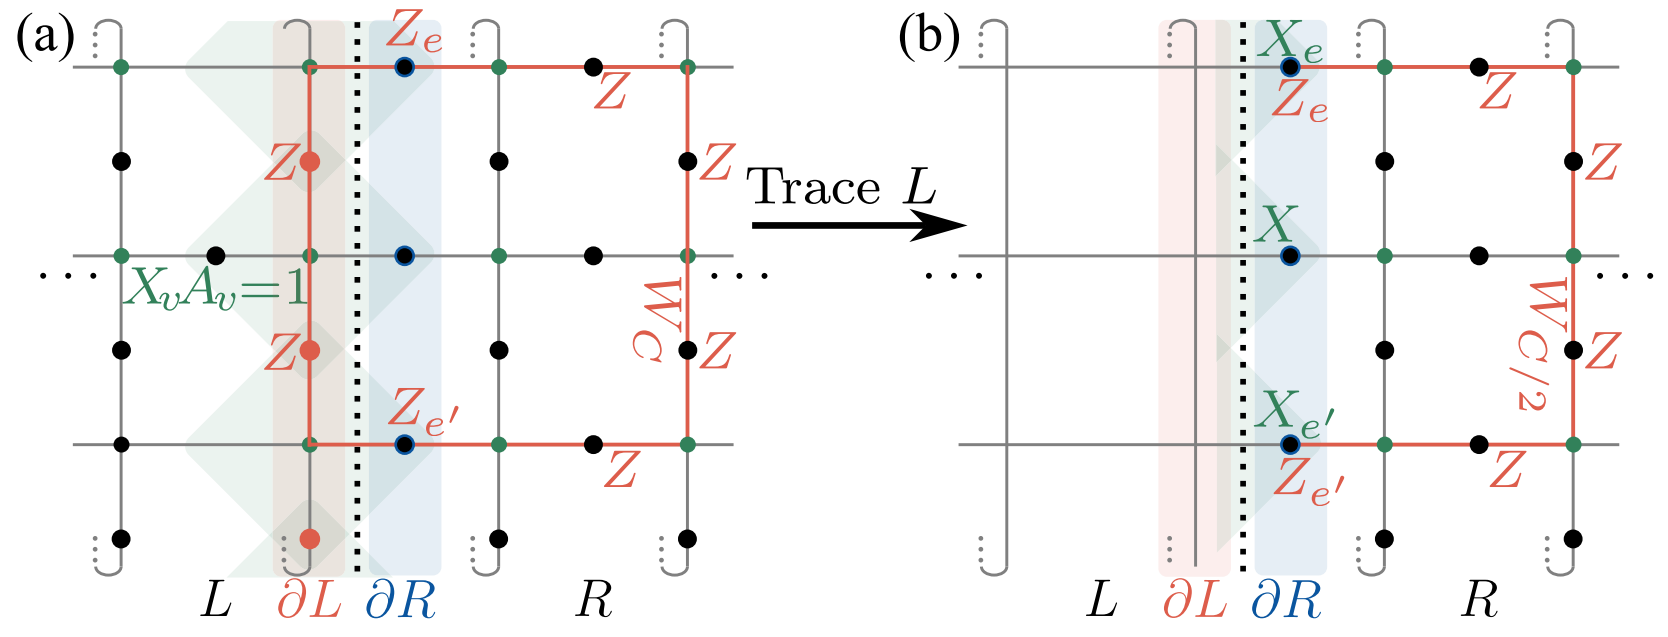
\includegraphics[height=0.12\textheight]{residual-gauss-law}
  \caption{(a) }\label{fig.basic-settings}
\end{figure}
The Hamiltonian of the Fradkin-Shenker model, the model that will be used in the demonstration of the entanglement spectrum (ES) degeneracy here, reads
\[
H_{\mrm{FS}} = -\sum_{v}X_v - \sum_{p}B_p - h_x\sum_{e}X_e - J\sum_{vev'}Z_v Z_e Z_v'
\]
where $e$ and $v$ stand for \emph{edges} and \emph{vertices} respectively; $B_p$'s are plaquette operators composed by $Z$-Pauli matrices surrounding the plaquette $p$
\[
\mathcal{H} = \mathcal{H}_V\otimes\mathcal{H}_E = \lrm{\bigotimes_{v}\lr{\mathbb{C}^2}_v}\otimes \lrm{\bigotimes_{e}\lr{\mathbb{C}^2}_e}
\]
\[
H_{\mrm{TC}} = -\sum_{v}A_v - \sum_{p}B_p - h_x\sum_{e}X_e - h_z\sum_{e}Z_e
\]
$H_{\mrm{TC}}:\mathcal{H}_{V}\to\mathcal{H}_{V}$ 
\[
U_{\mrm{CX}} = \prod_{\anglelr{ve}}\mrm{CX}_{ve}
\]
\[
\mrm{CX}_{ve} = \frac{\mathds{1}_v+Z_v}{2}\mathds{1}_e + \frac{\mathds{1}_v-Z_v}{2}X_e = \frac{\mathds{1}_e+X_e}{2}\mathds{1}_v + \frac{\mathds{1}_e-X_e}{2}X_v
\]
\[
V_\mrm{CX} = U_{\mrm{CX}}\prod_{v}\ket{+}_v
\]
\[
V^\dagger_{\mrm{CX}}V_{\mrm{CX}} = \mathds{1} \quad,\quad V_{\mrm{CX}}V^\dagger_{\mrm{CX}} = \prod_{v}\lr{\frac{\mathds{1}+X_vA_v}{2}}
\]
\[
\ket{\Psi_{\mrm{FS}}} = U_{\mrm{CX}}\lr{\ket{\Psi_{\mrm{TC}}}\otimes\prod_{v}\ket{+}_v} = V_{\mrm{CX}}\ket{\Psi_{\mrm{TC}}}
\]

\begin{align*}
  \rho_{\mrm{FS}} 
  &= V_{\mrm{CX}}\rho_{\mrm{TC}}V^\dagger_{\mrm{CX}} \\
  &= V_{\mrm{CX}}\lr{\frac{\mathds{1}+\tilde{W}_h}{2}} \lr{\frac{\mathds{1}+\tilde{W}_v}{2}} \prod_{v}\lr{\frac{\mathds{1}+A_v}{2}} \prod_{p}\lr{\frac{\mathds{1}+B_p}{2}} V^\dagger_{\mrm{CX}} 
\end{align*}

\section{Block-Diagonalization of the Density Matrix}
$[\rho_{\mrm{FS}},X_e]=0,\;\forall e\in\de R$

\section{Kitaev Model}
\subsection{Majorana Gauge Theory}
\subsection{Spin Language}

\begin{thebibliography}{99}
    \bibitem{PRX}\href{https://journals.aps.org/prx/abstract/10.1103/PhysRevX.15.011001}{Wen-Tao Xu, Tibor Rakovszky, Michael Knap, and Frank Pollmann, \emph{Entanglement Properties of Gauge Theories from Higher-Form Symmetries}, Phys. Rev. X \textbf{15}, 011001 (2025)}
\end{thebibliography}
\end{document}


 